\chapter{基于消息传递网络的复合物筛选模型}
\label{chapter:MPNN}
\section{引言}
\label{section:MPNN:Put}

模型\ref{section:NodeConv:Put}和模型\ref{section:EdgeConv:intro}分别是结点嵌入和邻边嵌入模型,蛋白质复合物的形成和蛋白质特征以及蛋白质互作特征均具有相关性。
无论普通的GCN模型还是EdgeConv模型,均只能直接基于结点特征进行卷积运算,或者邻边特征转换为结点特征之后再进行图卷积运算,这个过程将邻边特征均匀的分配给了其相邻的结点,在模型训练过程邻边作为独立的计算元素依旧缺乏针对邻边本身的更新。这种情形下,邻边特征只能作为结点特征的补充,无法与复合物互作网络动态的结合起来。

为了将邻边特征与结点特征整合到模型的动态参数更新中,本节基于消息传递网络(Message Passing Neural Network,简称MPNN)提出蛋白质复合物特征融合模型,同时处理蛋白质复合物子图中的结点数据和邻边数据,将生物数据、全局拓扑特征以及局部拓扑特征动态的融合起来。
\section{消息传递网络介绍}
\label{section:MPNN:intro}

MPNN网络是一种基于消息传递的图结构学习框架。不同于图卷积模型必须将特征绑定到结点,MPNN将图结构的特征当成消息,特征在结构中的流动被视为消息的传递。在此框架下,图卷积神经网络可以被当作MPNN的特例,是只传递结点消息的MPNN网络。


MPNN网络的具体实现如式\ref{equ:MPNNPassing}所示。

\begin{equation}
    \label{equ:MPNNPassing}
    m_v^{t+1} = \sum_{w \in N_{(v)}}M_t(h_v^t,h_w^t,e_{vw}^t)
\end{equation}
\begin{equation}
    \label{equ:MPNNReadout}
    h_v^{t+1} = U_t(h_v^t,m_v^{t+1})
\end{equation}
其中$N_{(v)}$表示图中结点$v$的邻居,$t$为时间步。公式\ref{equ:MPNNPassing}表示消息传递阶段(Message Passing),$M_t$表示消息传递的更新函数,代表结点w向结点v传递消息的过程中,其传递的消息$h_v^t,h_w^t,e_{vw}$的更新方式。公式\ref{equ:MPNNReadout}表示更新阶段,$U_t$表示更新阶段的函数,代表结点v汇总所有周围消息后的数据更新方式。


\section{基于消息传递网络的复合物筛选模型}
\label{section:MPNN:detail}

基于消息传递网络的复合物筛选模型是基于MPNN网络的改进。
为了使得结点特征和邻边特征具有融合的能力,蛋白质复合物特征融合模型中采用了结点更新邻边,邻边更新结点的方式。在每一层的MPNN过程中,结点t时刻特征更新为邻边t+1时刻特征、邻边t特征更新为结点t+1时刻特征。结点特征的更新具体方法如下所示,其中$Linear$为一层感知器。
\begin{equation}
    \label{equ:MineMPNNPassing}
    m_v^{t+1} = \sum_{w \in N_{(v)}}Linear^t(e_{vw}^t)
\end{equation}

\begin{equation}
    \label{equ:MineMPNNReadout}
    h_v^{t+1} = Max(h_v^t,m_v^{t+1})
\end{equation}
从式中可以看出,结点的特征更新来源分为两部分,其一为汇聚所有邻边的特征$e_{vw}^t$,同时为了保留一部分结点中具有关键性的原始特征,其更新方式采用了maxpool。邻边特征的具体更新方法如下所示。
\begin{equation}
    \label{equ:MineMPNNedge}
    e_{vw}^{t+1} = Max(e_{vw}^t,Linear_0^t(m_w^{l} - m_v^{l}) + Linear_1^t m_v^{l})
\end{equation}
从式中得出,类似于结点更新模型,邻边的特征更新也可以分为两部分,最后同样采用了maxpool的方式保留关键邻边特征。邻边特征的更新方式综合考虑了源点到汇点的特征流动部分$m_w^{l} - m_v^{l}$以及汇点的特征保留部分$m_v^{l}$。


最后融合模型同样考虑了复合物子图的整体拓扑特征,为通过图论计算的总体拓扑结构数据,作为不可学习的特征与MPNN读出的特征拼接到一起,作为最终的图特征输出。总体拓扑特征计算参考\cite{yu_predicting_2014}。

\section{算法具体实现与流程}
\label{section:MPNN:flow}

子图数据保留GO注释特征、拓扑域特征以及亚细胞定位特征等邻边特征,保留Deepwalk特征、GAE特征等结点特征。形成兼具结点和邻边特征的复合物特征子图数据,其中结点特征维度为82维,邻边特征维度维12维。

\begin{figure}[htbp]
    \centering
    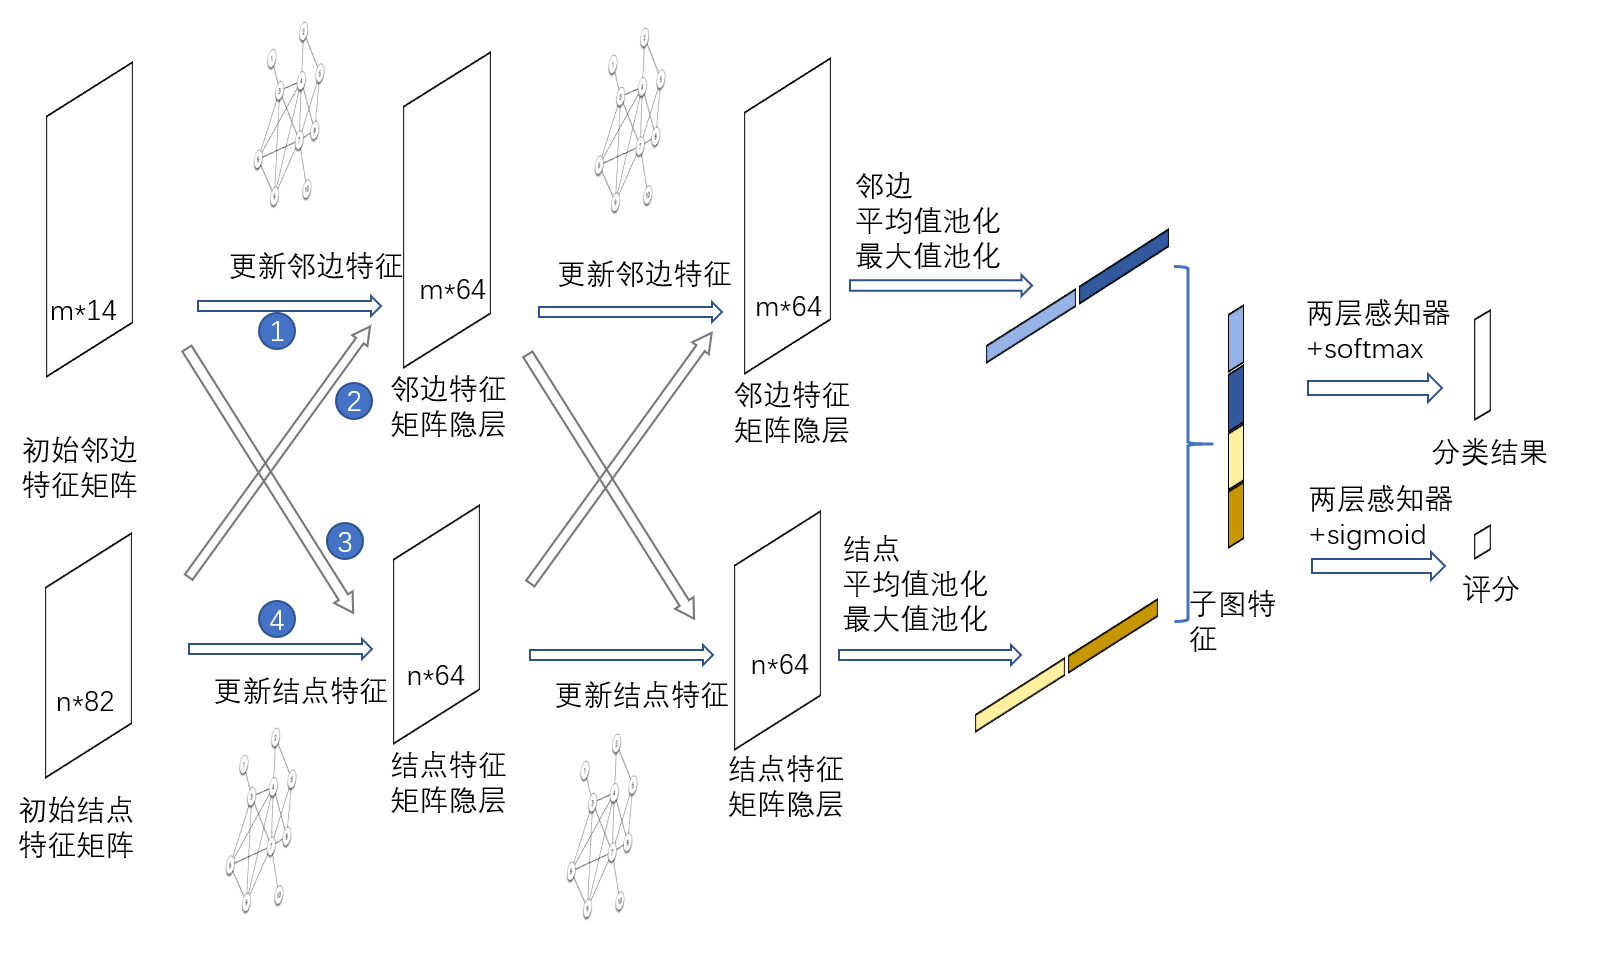
\includegraphics[width=14cm]{MPNN/flow}
    \caption{基于特征融合的分类模型总体流程}
    \label{fig:MPNN/flow}
\end{figure}

在模型中,添加了两层结点和邻边同时更新的MPNN网络,如图\ref{fig:MPNN/flow}所示。每一层MPNN网络中,结点特征更新由结点以及结点周围邻边特征共同确定,如示意图中的结点特征矩阵隐层的数据流所示,其具体的计算方法如公式\ref{equ:MineMPNNReadout}所示。邻边特征更新由邻边以及邻边两侧端点的结点特征共同确定,如示意图中的邻边特征矩阵隐层的数据流所示,其具体的计算方法如公式\ref{equ:MineMPNNedge}所示。

消息传递过程中隐层维度设置为64维,两层消息传递之后,采用了对结点特征Maxpool和MeanPool的池化方法以及对邻边Maxpool和MeanPool的池化方法。一共可以得出四个池化结果,对结果进行拼接之后,形成的256维的特征代表图整体特征。后续分别为两层感知器和softmax层得到图的分类预测,两层感知器和sigmoid层得到图的评分预测。

\section{实验设计及结果分析}
\label{section:MPNN:experience}
为了验证基于消息传递网络的模型的提升,本文对比了前两章分别设计的基于图卷积神经网络的复合物筛选模型和基于邻边卷积网络的复合物筛选模型。

基于图卷积神经网络的复合物筛选模型是基于研究蛋白质相互作用网络的拓扑结构展开,利用了结点的拓扑特征并基于结点的图卷积神经网络对拓扑特征进行融合,一定程度上体现了$PIN$网络中结点嵌入对复合物预测的作用,证实了复合物中蛋白质在互作网络中相关性对复合物的形成具有一定的影响。

基于邻边卷积网络的复合物筛选模型是基于研究蛋白质之间相似性特征展开,利用了邻边的相似性特征并基于邻边卷积对数据进行融合。生物的相似性数据对复合物预测以及复合物分类具有较明显的提升。

消息传递模型致力于向PIN网络全局特征以及生物特征融合到一起,分别以结点和邻边的形式嵌入到复合物子图中。相较于单独利用其中一方面的模型具有更好的预测能力。为了验证模型的有效性,本章进行了如下的实现。

实验在DIP和Biogrid网络中分别运行了Dpclus、Clique和IPCA三个复合物生成算法。实验结果如下所示。

图\ref{fig:result/DIP/fusion}为在DIP网络中,基于结点的全局特征模型、基于邻边的生物特征模型以及特征融合模型筛选之后结果的对比。
\begin{figure}[htbp]
    \centering
    \subcaptionbox{F1值对比}{\label{fig:result/DIP/F1/fusion}
        \includegraphics[width=10cm]{result/DIP/F1/fusion}}
    \vskip0.2cm
    \subcaptionbox{SPA值对比}{\label{fig:result/DIP/SPA/fusion}
        \includegraphics[width=10cm]{result/DIP/SPA/fusion}}
    \caption{DIP网络不同模型处理后结果对比}
    \label{fig:result/DIP/fusion}
\end{figure}

从图中可以看出,在DIP网络中,MPNN融合模型在F1的结果中取得了较大的提升,在Dpclus和Clique的数据样本中均得到了最优结果。

图\ref{fig:result/Biogrid/fusion}为在Biogrid网络中,基于结点的全局特征模型、基于邻边的生物特征模型以及特征融合模型筛选之后结果的对比。
\begin{figure}[htbp]
    \centering
    \subcaptionbox{F1值对比}{\label{fig:result/Biogrid/F1/fusion}
        \includegraphics[width=10cm]{result/Biogrid/F1/fusion}}
    \vskip0.2cm
    \subcaptionbox{SPA值对比}{\label{fig:result/Biogrid/SPA/fusion}
        \includegraphics[width=10cm]{result/Biogrid/SPA/fusion}}
    \caption{Biogrid网络不同模型处理后结果对比}
    \label{fig:result/Biogrid/fusion}
\end{figure}
从图中可以看出,在Clique样本集上,其综合评价指标和F1值均达到了最优结果。而在Dpclus的样本集中,综合评价指标也得到了最优结果。


\section{本章小结}
\label{section:MPNN:summary}

本章基于特征融合出发,探讨了融合$PIN$全局特征以及生物相似性特征的情况下,模型设计以及进行了相关的实验。
在特征子图具有GAE和Deepwalk特征等结点特征、多种蛋白质相似性嵌入邻居特征的情况下,本章提出了改进的MPNN更新方法。提出了结点与邻边交替融合更新的模型。最后本章对比了利用结点特征的基于图卷积的模型,利用相似性特征的基于邻边卷积的模型,实验结果表明融合方法对于数据集中的结果具有一定的提升效果。